\documentclass[12pt, a4paper]{third-rep}

% colours
\usepackage[table]{xcolor}
\definecolor{mydarkblue}{rgb}{0,0.08,0.45}
\definecolor{mintbg}{rgb}{0.95,0.95,0.95}
\definecolor{listingframe}{rgb}{1,0.31,0}

% tcolorbox my beloved
\usepackage{tcolorbox}
\tcbuselibrary{skins,listings,raster,minted,breakable}
\newtcbinputlisting[auto counter]{\pythoncode}[3][]{
  enhanced jigsaw,breakable,
  boxrule=0.2mm,top=1mm,bottom=1mm,left=1mm,right=1mm,
  before=\par\smallskip,after=\par\smallskip,
  listing file={#3},
  listing only,
  listing engine=minted,
  minted language=python,
  minted style=colorful,
  colback=mintbg,
  colframe=listingframe,
  fonttitle=\bfseries,
  title={Listing \thetcbcounter: #2},
  #1
}

% graphics
\usepackage{graphicx}
\graphicspath{ {assets/} }

% minted replaces listings
% \usepackage[cachedir=\detokenize{latex.out/minted}]{minted}
\usepackage{minted}
\usepackage{dingbat}
\setminted[python]{
    breaklines,
    breakanywhere,
    autogobble,
}

% hyperlink setup
\usepackage{url}
\usepackage{hyperref}
\hypersetup{
    pdftitle={},
    pdfsubject={},
    pdfkeywords={},
    pdfborder=0 0 0,
    pdfpagemode=UseNone,
    colorlinks=true,
    linkcolor=mydarkblue,
    citecolor=mydarkblue,
    filecolor=mydarkblue,
    urlcolor=mydarkblue,
}

% provides the ability it strikethrough things
\usepackage{cancel}
\newcommand\hcancel[2][red]{
  \setbox0=\hbox{$#2$}\rlap{
    \raisebox{.45\ht0}{\textcolor{#1}{\rule{\wd0}{1pt}}}
  }#2
}

% used for nesting figures
\usepackage{subcaption}

% Maths/CS symbols
\usepackage{stmaryrd}
\usepackage{amsmath}
\usepackage{amssymb}
\usepackage{amsfonts}

% booktabs makes tables better
\usepackage{booktabs}
\captionsetup[table]{hypcap=false}

% biblatex stuff
\usepackage[style=alphabetic,natbib]{biblatex}
\addbibresource{refs.bib}

% package for defining custom math symbols
\usepackage{stackengine}
\stackMath
\newcommand{\cryptoSample}{\shortleftarrow\kern-1.5ex\text{\scriptsize \$}}

%% Uncomment the following lines if you want to include the date as a
%% header in draft versions. See the documentation for fancyhdr for
%% more ways of modifying headers (texdoc fancyhdr will show you the
%% docs) 

% \usepackage{fancyhdr}
% \setlength{\headheight}{14.5pt} % silence warnings
% \pagestyle{fancy}
% \lhead{}  % left head
% \chead{Draft: \today} % centre head
% \lfoot{}
% \cfoot{\thepage}
% \rfoot{}

% title stuff
\usepackage{titlesec}
\newcommand{\PreContentTitleFormat}{
  \titleformat{\chapter}[display]{\scshape\Large}
  {\Large\filleft\MakeUppercase{\chaptertitlename} \Huge\thechapter}
  {1ex}
  {}
[\vspace{1ex}\titlerule]}

\newcommand{\ContentTitleFormat}{
  \titleformat{\chapter}[display]{\scshape\huge}
  {\Large\filleft\MakeUppercase{\chaptertitlename} \Huge\thechapter}
  {1ex}
  {\titlerule\vspace{1ex}\filright}
  [\vspace{1ex}\titlerule]
}

% glossary stuff
\usepackage[toc]{glossaries}
\setacronymstyle{long-short}
\loadglsentries{glossary}
\makenoidxglossaries{}

% Tikz stuff
\usepackage{tikz}
\usepackage{tikzpeople}

% plotting things
\usepackage{pgfplots}
\pgfplotsset{compat=1.18}
\usetikzlibrary{intersections,decorations.markings}

\newcommand{\plotcurve}[3][thick, every plot/.style={smooth}]{
  % plot curve y^2 = x^3 + a x + b in range [-3,3]^2
  % parameter 1 (optional): style options for curve (color, etc)
  % parameter 2: curve parameter a
  % parameter 3: curve parameter b
  \draw[gray] (-3,-3) rectangle (3,3);
  \draw[->,>=latex,gray] (-3,0) -- (3,0);
  \draw[->,>=latex,gray] (0,-3) -- (0,3);
  \draw[name path=curve, #1] plot[id=curve#2#3, raw gnuplot] function {
    f(x,y) = y**2 - x**3 - #2*x - #3;
    set xrange [-3:3];
    set yrange [-3:3];
    set view 0,0;
    set isosample 50,50;
    set cont base;
    set cntrparam levels incre 0,0.1,0;
    unset surface;
    splot f(x,y);
  };
}

\tikzset{
  tangent/.style={
    decoration={markings, mark=at position #1 with {
      \coordinate (tangent point-\pgfkeysvalueof{/pgf/decoration/mark info/sequence number}) at (0pt,0pt);
      \coordinate (tangent unit vector-\pgfkeysvalueof{/pgf/decoration/mark info/sequence number}) at (1,0pt);
      \coordinate (tangent orthogonal unit vector-\pgfkeysvalueof{/pgf/decoration/mark info/sequence number}) at (0pt,1);
    }},
    postaction=decorate
  },
  use tangent/.style={
    shift=(tangent point-#1),
    x=(tangent unit vector-#1),
    y=(tangent orthogonal unit vector-#1)
  },
  use tangent/.default=1
}

% crypgraphy stuff
\usepackage[operators, sets]{cryptocode}
\newcommand{\mathAdded}[1]{\textcolor{green!60!gray}{\mathbf{#1}}}
\newcommand{\textAdded}[1]{\textcolor{green!60!gray}{\textbf{#1}}}

% cleverly decides how to reference a given ref
% must be loaded after hyperref and amsmath
\usepackage{cleveref}

% only work on a chapter at a time to improve compile times
% \includeonly{chapter1,appendix1,appendix2}

% specify how the document should handle hyphenation at page borders
\tolerance=1
\emergencystretch=\maxdimen
\hbadness=10000

\title{Exploring Password-Authenticated Key-Exchange Algorithms}
\author{Sam Leonard}
\supervisor{Professor Bernardo Magri}
\reportyear{2023}
\studentid{f41751sl}

\abstractfile{abstract.tex}
\thanksfile{merci.tex}

\begin{document}
\PreContentTitleFormat

\dotitleandabstract

%% Generate contents etc
\tableofcontents

%% These include the actual text
\ContentTitleFormat
\chapter{Context}
\section{Background on PAKEs}
\subsection{What is a PAKE?}
\glspl{pake} are interactive, two party cryptographic protocols where each party shares knowledge of a password (a low entropy secret) and seeks to obtain a strong shared key e.g. for use later with a symmetric cipher. Critically an eavesdropper who can listen in two all messages of the key negotiation cannot learn enough information to bruteforce the password. Another way of phrasing this is that brute force attacks on the key must be "\glslink{ocrypto}{online}".

\medskip
There are two main types of \gls{pake} algorithm - \glspl{apake} and \glspl{bpake}.
\begin{itemize}
  \item \glspl{bpake} are \glspl{pake} where both parties share knowledge of the same secret password.
  \item \glspl{apake} are \glspl{pake} where one party has the password and the other has a "\gls{veri}" which is computed via a one-way function from the secret password.
\end{itemize}

\begin{figure}[H]
  \centering
  \begin{tikzpicture}
    \node[alice,minimum size=1.5cm] at (0,0) {Alice};
    \node[scale=0.03] at (1,0.5) {\includegraphics{key.png}};
    \node[bob,mirrored,minimum size=1.5cm] at (5,0) {Bob};
    \node[scale=0.03] at (4,0.5) {\includegraphics{key.png}};
    \node[alice,minimum size=1.5cm] at (7,0) {Alice};
    \node[scale=0.03] at (8,0.5) {\includegraphics{key.png}};
    \node[bob,mirrored,minimum size=1.5cm] at (12,0) {Bob};
    \node[scale=0.03] at (11,0.5) {\includegraphics{shuffled_key.png}};
    \draw (6,1.3) -- (6,-2.3);
    \draw (2.5,-2) node {Balanced PAKE};
    \draw (9.5,-2) node {Augmented PAKE};
  \end{tikzpicture}

  \caption{An illustration of the difference between \glspl{apake} and \glspl{bpake}}
  \label{fig:pake_compare}
\end{figure}

\clearpage

\subsection{A brief history of PAKE algorithms}
The first \gls{pake} algorithm was Bellovin and Merritt's \gls{eke} scheme \cite{eke}.
It works using a mix of \gls{symcrypto} and \gls{asymcrypto} to perform a key exchange.
This comes with many challenges and subtle mistakes that are easy to make;
primarily for the security of the system whatever is encrypted by the shared secret key(P) must be indistinguishable from random data.
Otherwise an attacker can determine whether their guess at a trial decryption is valid.
The \gls{rsa} variant of \gls{eke} has this issue - the \gls{rsa} parameter $e$ is what is encrypted and sent in the first message.
For \gls{rsa} all valid values of $e$ are odd, so this would prevent it being used.
This is solved by adding $1$ to $e$ with a $50\%$ chance.
\Cref{fig:eke-rsa} shows this protocol in full. While many of the initial variants on \gls{eke} have been shown to flawed/vulnerable, later variants have made it into real world use, such as in \gls{eap} \cite{eap} where it is available as \gls{eap}-\gls{eke} \cite{eap-eke}.
In \cref{chap:appendix-eke} you can find a Python implementation of this scheme

\subsubsection{An Aside on Notation}
\begin{itemize}
  \item $\shortleftarrow$: Assignment - $x \shortleftarrow \ 5$ means x is assigned a value of 5.
  \item $\cryptoSample$: Sampling from a given set - $x \cryptoSample \ \mathbb{R}$ means to choose $x$ at random from the set of real numbers.
\end{itemize}

\begin{figure}[H]
  \centering

  \begin{tabular}{ |c|c|l| }
    \hline
    Shared Parameter & Secret & Explanation \\
    \hline
    $P$ & yes & the shared password \\ \hline
  \end{tabular}

  \caption{\gls{eke} shared parameters}
  \label{fig:eke-shared-params}
\end{figure}

\begin{figure}[H]
  \pseudocodeblock[head=EKE-RSA]{
    \textbf{Alice} \< \< \textbf{Bob} \\[0.1\baselineskip][\hline]
    \< \< \\[-0.5\baselineskip]
    Ea \gets (e, n) \< \< \\
    b \sample \bin \< \sendmessageright*{A,P(e + b),n} \< Ea \gets (e, n)\\ 
    challenge_A \sample \ZZ_n \< \sendmessageleft*{P(Ea(R))} \< R \sample \text{Keyspace}\\ 
    \< \sendmessageright*{R(challenge_A)} \< challenge_B \sample \ZZ_n \\
    \text{verify } challenge_A \< \sendmessageleft*{R(challenge_A, challenge_B)} \< \\
    \< \sendmessageright*{R(challenge_B)} \< \text{verify } challenge_B
  }

  \caption{Implementing \gls{eke} using \gls{rsa}}
  \label{fig:eke-rsa}
\end{figure}

\clearpage

\subsubsection{SPAKE}
\glslink{spake}{SPAKE1} and \glslink{spake}{SPAKE2} are \glspl{bpake}' which were introduced slightly later on by Michel Abdalla and David Pointcheval \cite{spake} as variations on \gls{eke}.
They are very similar so we will just explore \glslink{spake}{SPAKE2} as we are more interested in \glslink{ocrypto}{online} algorithms.
\gls{spake} differs from EKE in the following ways:

\begin{enumerate}
  \item The encryption function is replaced by a simple one-time pad.
  \item The \gls{asymcrypto} is provided by \gls{dh}
  \item There is no explicit mutual authentication phase where challenges are exchanged.
    This has the advantage of reducing the number of messages that need to be sent.
\end{enumerate}

\begin{figure}[H]
  \centering

  \begin{tabular}{ |c|c|p{0.6\linewidth}| }
    \hline
    Shared Parameter & Secret & Explanation \\
    \hline
    $pw$ & yes & the shared password encoded as an element of $\ZZ_p$ \\ \hline
    $\GG$ & no & the mathematical group in which we will perform all opertions \\  \hline
    $g$ & no & the generator of $\GG$ \\ \hline
    $p$ & no & the \gls{safeprime} which defines the finite field for all operations in $\GG$ \\ \hline
    $M$ & no & an element in $\GG$ associated with user $A$ \\ \hline
    $N$ & no & an element in $\GG$ associated with user $B$ \\ \hline
    $H$ & no & a secure hash function \\ \hline
  \end{tabular}

  \caption{\gls{spake} shared parameters}
  \label{fig:spake-shared-params}
\end{figure}

\begin{figure}[H]
  \pseudocodeblock[head=SPAKE2]{
    \textbf{Alice} \< \< \textbf{Bob} \\[0.1\baselineskip][\hline]
    \< \< \\[-0.5\baselineskip]
    x \sample \ZZ_p \< \< y \sample \ZZ_p \\
    X \gets g^x \< \< Y \gets g^y \\
    X^* \gets X \cdot M^{pw} \< \< Y^* \gets X \cdot N^{pw} \\
    \< \sendmessageright*{X^*} \< \\
    \< \sendmessageleft*{Y^*} \< \\
    K_A \gets (Y^* / N^{pw})^x \< \< K_B \gets (X^* / M^{pw})^y \\
    SK_A \gets H(A, B, X^*, Y^*, Ka) \< \< SK_B \gets H(A, B, X^*, Y^*, Kb)
  }

  \caption{SPAKE2 Protocol}
  \label{fig:spake2}
\end{figure}

\clearpage

\subsubsection{SRP}
Finally we will look at \gls{srp} an \gls{apake} first published in 1998, unlike \glslink{spake}{SPAKE2} it is not a modification of \gls{eke}.
\gls{srp} has gone through many revisions, at time of writing \glslink{srp}{SRP6a} is the latest version.
\gls{srp} is likely the most used \gls{pake} protocol in the world due to it's use in Apple's iCloud Keychain \cite{apple-keychain-srp} and it's availability as a \gls{tls} ciphersuite \cite{tls-srp}.
However it is quite weird for what it does and there is no security proof for it \cite{srp-blog}. An implementation of the protocol in Python can be found in \cref{chap:appendix-srp}.

\begin{figure}[H]
  \centering

  \begin{tabular}{ |c|c|p{0.7\linewidth}| }
    \hline
    Parameter & Secret & Explanation \\
    \hline
    $v$ & yes & the \gls{veri}\label{text:srp-verifier-generation} stored by the server: $v=g^{H(s,I,P)}$ \\ \hline
    $P$ & yes & the user's password \\ \hline
    $I$ & no & the user's name \\ \hline
    $g$ & no & the generator of $\GG$ \\ \hline
    $p$ & no & the \gls{safeprime} which defines the finite field for all operations in $\GG$ \\ \hline
    $H$ & no & a secure hash function \\ \hline
  \end{tabular}

  \caption{\gls{srp} parameters}
  \label{fig:srp-shared-params}
\end{figure}

\begin{figure}[H]
  \pseudocodeblock[head=SRP]{
    \textbf{Alice} \< \< \textbf{Bob} \\[0.1\baselineskip][\hline]
    \< \< \\[-0.5\baselineskip]
    a \sample \{1 \dots n - 1\} \< \sendmessageright*{I} \< s,v \gets \text{lookup}(I)\\
    x \gets H(s, I, P) \< \sendmessageleft*{s} \< b \sample \{1 \dots n - 1\}\\
    A \gets g^a \< \sendmessageright*{A} \< B \gets 3v + g^b \\
    u \gets H(A, B) \< \sendmessageleft*{B} \< u \gets H(A, B)\\
    S \gets (B - 3g^x)^{a+ux}\< \< S \gets (Av^u)^b\\
    M_1 \gets H(A,B,S) \< \sendmessageright*{M_1} \< \text{verify } M_1\\
    \text{verify } M_2 \< \sendmessageleft*{M_2} \< M_2 \gets H(A,M_1,S)\\
    K \gets H(s)\< \< K \gets H(S)
  }

  \caption{SRP-6 Protocol}
  \label{fig:srp}
\end{figure}

\clearpage

\section{Elliptic Curve Cryptography}
Many modern Cryptograhpic protocols make use of a mathematical object known as an elliptic curve.
First proposed in 1985 independently by Neal Koblitz \cite{ecc-first-use-koblitz} and Victor S. Miller \cite{ecc-first-use-miller}.
Elliptic curves are attractive to cryptographers as they maintain a very high level of strength at smaller key sizes, this allows for protocols to consume less bandwidth, less memory and execute faster \cite{state-of-ecc}.
To illustrate just how great the size savings are - \gls{nist} suggests that an elliptic curve key of just 256 bits provides the same level of security as an \gls{rsa} key of 3072 bits \cite{nist-ecc-reqs}.

\subsection{But what actually is an elliptic curve?}
With regards to Cryptography elliptic curves tend to come in one of two forms:
\begin{itemize}
  \item Short Weierstra\ss{} Form: $y^2 = x^3 + ax + b$
  \item Montgomery Form: $by^2 = x^3 + ax^2 + x$
\end{itemize}

\begin{figure}[H]
  \centering
  \begin{tikzpicture}[thick,>=latex]
    \begin{scope}
      \draw[<->,gray] (-3,0) -- (3,0) node[right] {$x \in \mathbb{R}$};
      \draw[<->,gray] (0,-3) -- (0,3) node[above] {$y \in \mathbb{R}$};
      \draw[thick, name path=curve, every plot/.style={smooth}] plot[id=weierstrass-curve-1, raw gnuplot] function {
        f(x,y) = y**2 - (x**3 - 2.5*x + 1);
        set xrange [-3:3];
        set yrange [-3:3];
        set view 0,0;
        set isosample 50,50;
        set cont base;
        set cntrparam levels incre 0,0.1,0;
        unset surface;
        splot f(x,y);
      };
    \end{scope}

    \node at (0,-4) {$y^2 = x^3 - 2 x - 1$ over $\mathbb{R}$};
    \node at (0,-5) {Short Weierstra\ss{} Form};

    \begin{scope}[shift={(8,0)}]
      \draw[<->,gray] (-3,0) -- (3,0) node[right] {$x \in \mathbb{R}$};
      \draw[<->,gray] (0,-3) -- (0,3) node[above] {$y \in \mathbb{R}$};
      \draw[thick, name path=curve, every plot/.style={smooth}] plot[id=montgomery-curve-1, raw gnuplot] function {
        f(x,y) = 2*y**2 - (x**3 - 3*x - x);
        set xrange [-3:3];
        set yrange [-3:3];
        set view 0,0;
        set isosample 50,50;
        set cont base;
        set cntrparam levels incre 0,0.1,0;
        unset surface;
        splot f(x,y);
      };
    \end{scope}

    \node at (8,-4) {$2 y^2 = x^3 - 3 x^2 - x$ over $\mathbb{R}$};
    \node at (8,-5) {Montgomery Form};
  \end{tikzpicture}

  \caption{Elliptic curves over $\RR$, Adapted from TikZ for Cryptographers \cite{tikz-crypto}}
\end{figure}

Weierstra\ss{} form is special as it is the general case for all elliptic curves, meaning all elliptic curves can be expressed as a Weierstra\ss{} curve.
This property means that it is commonly used for expressing various curves.
Montgomery form isn't quite as flexible, however it is favourable because it leads to significantly faster multiplication and addition operations via Montgomery's ladder \cite{montgom-ladder}.

\subsection{How do we do Cryptography with curves?}
To perform Cryptography with elliptic curves we need to define an "\gls{abgroup}" to work in.
An \gls{abgroup} is a group whose group operation is also commutative, for example the addition operator over the integers: ($+$, $\ZZ$) is an \gls{abgroup}.
\glspl{abgroup} form the basis of many modern Cryptographic algorithms, a \gls{dh} key exchange can be performed in any \gls{abgroup} for instance.

Our \gls{abgroup} is built on the idea of "adding" points on the curve.
To add two points, we find the line which passes through our two points and we continue along that line until we hit our curve again.
We then reflect this point in the $x$-axis to get our result.
What if we want to add our point to itself? Now there isn't a unique line through one point, however we are making the rules so in this case we will take the tangent to the curve at that point and then we can treat it the same as before.
What if our line doesn't intersect with the curve? In this case we define a new point called the "neutral element" - $\mathcal{O}$.
It is also called the point at infinity as it can be considered to be the single point at the end of every vertical line at infinity.
\Cref{fig:point-add-rules} illustrates all of these rules and edge cases.

\begin{figure}[H]
  \centering
  \begin{tikzpicture}[scale=.555]

    \begin{scope}[xshift=0cm]
      \plotcurve{-2}{2}
      \draw[->, >=latex, thick] (-2.5,-1) -- ++(0,3.5) node[right] {$\mathcal{O}$};
      \node[below] at (0,-4) {Neutral element $\mathcal{O}$};
    \end{scope}

    \begin{scope}[xshift=7.5cm]
      \plotcurve{-2}{2}
      \draw[dashed, semithick, name path=vertical] (-1.25,2.5) -- ++(0,-5);
      \draw[name intersections={of=curve and vertical}] (intersection-1) node {$\bullet$} node[above left] {$P$}
      (intersection-2) node {$\bullet$} node[below left] {$-P$};
      \node[below] at (0,-4) {Inverse element $-P$};
    \end{scope}

    \begin{scope}[xshift=15cm]
      \plotcurve{-2}{2}
      \draw[thick, name path=chord] (-2.5,.5) -- (2.5,2.0);
      \draw[name intersections={of=curve and chord}] (intersection-1) node {$\bullet$} node[above left] {$P$}
      (intersection-2) node {$\bullet$} node[above right=-1pt] {$Q$}
      (intersection-3) node {$\bullet$} coordinate[name=mPQ];
      \draw[dashed, semithick, name path=vertical] (mPQ) ++(0,1) -- +(0,-5.5);
      \draw[name intersections={of=curve and vertical}] (intersection-2) node {$\bullet$} node[below left] {$P+Q$};
      \node[below, align=center] at (0,-4) {Addition $P+Q$ \\ ``Chord rule''};
    \end{scope}

    \begin{scope}[xshift=22.5cm]
      \plotcurve[thick, tangent=0.265, every plot/.style={sharp plot}]{-2}{2}
      \draw[thick, use tangent, name path=chord] (-.6,0) -- (1.5,0);
      \draw[name intersections={of=curve and chord}] (intersection-1) node {$\bullet$} node[above] {$P$}
      (intersection-2) node {$\bullet$} coordinate[name=mPQ];
      \draw[dashed, semithick, name path=vertical] (mPQ) ++(0,1) -- +(0,-5.0);
      \draw[name intersections={of=curve and vertical}] (intersection-2) node {$\bullet$} node[below left] {$2P$};
      \node[below, align=center] at (0,-4) {Doubling $P+P$ \\ ``Tangent rule''};
    \end{scope}

  \end{tikzpicture}
  \caption{Elliptic Curve Group Operations, reproduced from TikZ for Cryptographers \cite{tikz-crypto}}
  \label{fig:point-add-rules}
\end{figure}

However it's not quite that simple for us. We cannot use $\RR$ as computers only have finite resources we need a finite set to work in. Instead we define our operations over a \gls{ff}, we will use the \gls{ff} of the integers mod a prime, denoted $\ZZ_p$ for some prime $p$. Lets take a look at what our finite fields look like in a small finite field - $\ZZ_{89}$. \begin{figure}[H]
  \centering

  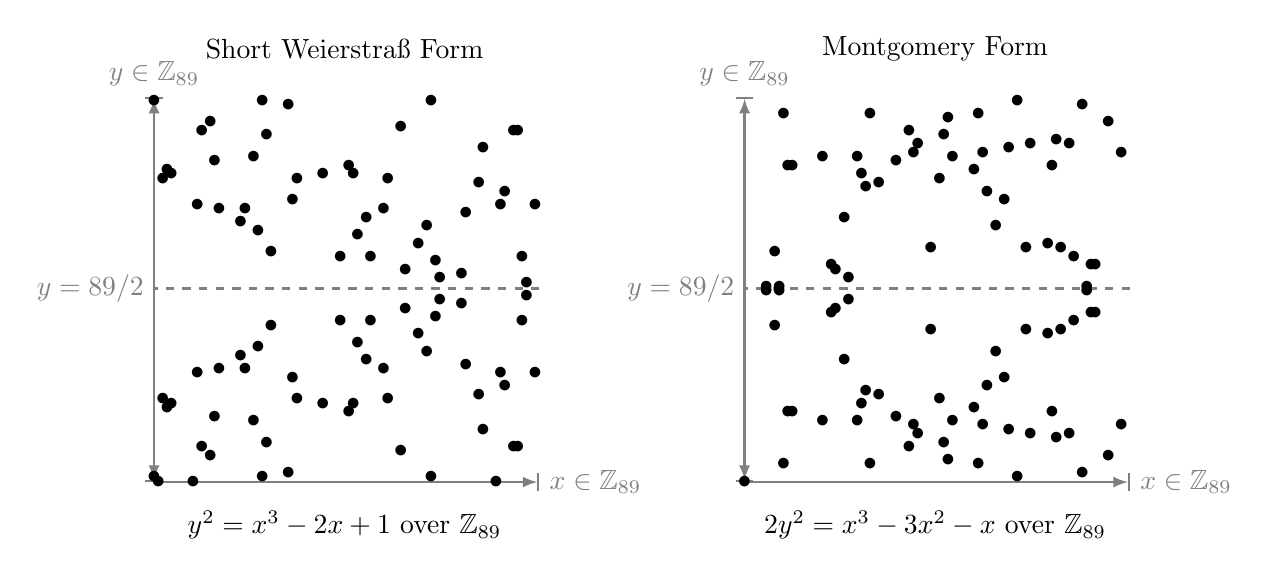
\begin{tikzpicture}[thick,>=latex]
    % Generate list of points with Sage:
    % sage: E = EllipticCurve(Integers(89), [-2,1])
    % sage: points = {tuple(p)[:2] for p in E.points()}
    % sage: print(points)
    \begin{scope}[scale=.055]
      \draw[|<->|,gray] (0,0) -- (0,89) node[above] {$y \in \mathbb{Z}_{89}$};
      \draw[->|,gray] (0,0) -- (89,0) node[right] {$x \in \mathbb{Z}_{89}$};
      % weirdness to make the line actually split the plane
      \draw[dashed,gray] (89,44.7) -- (0,44.7) node[left] {$y = 89/2$};
      \foreach \point in {
        (43, 37), (50, 52), (72, 27), (20, 29), (58, 40), (58, 49), (14, 15), (27, 36), (13, 83), (26, 80), (47, 57), (65, 38), (3, 72), (3, 17), (24, 58), (33, 70), (26, 9), (84, 8), (54, 19), (45, 16), (85, 52), (14, 74), (4, 18), (75, 69), (45, 73), (65, 51), (86, 46), (49, 61), (33, 19), (81, 22), (39, 71), (25, 88), (9, 0), (79, 0), (50, 37), (2, 70), (53, 63), (20, 60), (27, 53), (39, 18), (84, 81), (31, 87), (43, 52), (80, 25), (1, 0), (25, 1), (15, 63), (76, 12), (64, 1), (63, 30), (66, 47), (80, 64), (83, 8), (72, 62), (88, 25), (2, 19), (21, 63), (23, 14), (21, 26), (64, 88), (32, 65), (71, 48), (88, 64), (81, 67), (10, 25), (31, 2), (0, 88), (85, 37), (66, 42), (61, 55), (53, 26), (71, 41), (10, 64), (11, 8), (75, 20), (11, 81), (32, 24), (54, 70), (15, 26), (49, 28), (0, 1), (83, 81), (57, 7), (86, 43), (46, 71), (24, 31), (23, 75), (4, 71), (47, 32), (76, 77), (13, 6), (63, 59), (46, 18), (61, 34), (57, 82)
      } {\node at \point {$\bullet$};}
      \node at (44, 100) {Short Weierstra\ss{} Form};
      \node at (44,-10) {$y^2 = x^3 - 2 x + 1$ over $\mathbb{Z}_{89}$};
    \end{scope}

    % Generate list of points with Python:
    % >>> f=lambda x,y: (int(2 * y**2) % 89) == ((x**3 -3*(x**2) - x) % 89)
    % >>> # yes this is suspect as fuck but it all works because modular arithmetic 🙃
    % >>> points = {(x,y) for x in range(89) for y in range(89) if f(x,y)}
    % >>> print(points)
    \begin{scope}[xshift=7.5cm,scale=.055]
      \draw[|<->|,gray] (0,0) -- (0,89) node[above] {$y \in \mathbb{Z}_{89}$};
      \draw[->|,gray] (0,0) -- (89,0) node[right] {$x \in \mathbb{Z}_{89}$};
      % weirdness to make the line actually split the plane
      \draw[dashed,gray] (89,44.7) -- (0,44.7) node[left] {$y = 89/2$};
      \foreach \point in {
        (70, 55), (24, 42), (81, 39), (45, 19), (73, 35), (76, 52), (28, 21), (66, 78), (29, 4), (26, 14), (23, 61), (55, 13), (56, 67), (79, 44), (65, 54), (11, 16), (35, 74), (84, 6), (0, 0), (47, 84), (11, 73), (9, 85), (70, 34), (18, 14), (72, 79), (87, 13), (39, 76), (66, 11), (75, 78), (7, 53), (26, 75), (8, 45), (63, 88), (54, 85), (81, 50), (58, 30), (80, 39), (72, 10), (65, 35), (28, 68), (63, 1), (18, 75), (53, 72), (76, 37), (31, 69), (23, 28), (61, 12), (75, 11), (21, 40), (21, 49), (48, 14), (71, 16), (45, 70), (84, 83), (43, 54), (71, 73), (39, 13), (5, 45), (8, 44), (29, 85), (55, 76), (7, 36), (78, 87), (20, 39), (10, 16), (73, 54), (38, 8), (54, 4), (80, 50), (38, 81), (40, 78), (58, 59), (31, 20), (53, 17), (60, 65), (79, 45), (27, 71), (56, 22), (10, 73), (20, 50), (48, 75), (87, 76), (24, 47), (9, 4), (27, 18), (60, 24), (46, 80), (43, 35), (78, 2), (47, 5), (61, 77), (46, 9), (35, 15), (5, 44), (40, 11)
      } {\node at \point {$\bullet$};}
      \node at (44,100) {Montgomery Form};
      \node at (44,-10) {$2y^2 = x^3 - 3x^2 - x$ over $\mathbb{Z}_{89}$};
    \end{scope}
  \end{tikzpicture}

  \caption{Elliptic curves over $\ZZ_{89}$, Adapted from TikZ for Cryptographers \cite{tikz-crypto}}
  \label{fig:ellip-curve-ff}
\end{figure}

This now looks very different to when we were looking at them in $\RR$, however it shows very clearly what the elements of our set look like.
They are points in the 2d coordinate plane with a symmetry around $p/2$.
This might not feel intuitive but it is actually exactly what we should expect to happen, in our finite field when we negate our point's y coordinate, instead of flipping it around the y-axis, our points get wrapped around $y=p$.
Hence our new point is the same distance from $y=p$ as our first point was with $y=0$, this is where our symmetry arises.

\subsection{Where can Elliptic Curve Cryptography go wrong?}
There are many attacks against various aspects of Elliptic Curves, in general they fall into the following categories:
\begin{itemize}
  \begin{item}
    Attacks against the \gls{ecdlp} security of the curve:
    \begin{itemize}
      \item{The rho method \cite{pollard-rho}}
      \item{Transfer Security \cite{multiplicative-transfer-attack,additive-transfer-attack}}
      \item{CM Field Discriminants \cite{safecurves}}
      \item{Curve Rigidity \cite{curve-rigidity}}
    \end{itemize}
  \end{item}
  \begin{item}
    Attacks against the concrete implementation of \gls{ecc}:
    \begin{itemize}
      \item{Ladders required for safe and fast point-scalar multiplication \cite{safecurves}}
      \item{Twist Security \cite{small-subgroup-attack,invalid-curve-attack}}
      \item{Completeness \cite{completeness-attack}}
      \item{Indistinguishability \cite{elligator2}}
    \end{itemize}
  \end{item}
\end{itemize}

All of these attacks individually can weaken or even break the security of a given cryptosystem if not accounted for.
However choosing the right curve is a good step in the right direction and can mitigate many of the attacks listed above.

\section{Modern PAKEs}
Recently many novel \glspl{pake} algorithms have been published, this is partly due to a request from the \gls{ietf} for the \gls{irtf} \gls{cfrg} to carry out a selection process to choose a \gls{pake} for usage in \gls{ietf} protocols.
That process concluded in 2020 with \gls{cpace} and \gls{opaque} being chosen as the recommended \gls{bpake} and \gls{apake} respectively \cite{cfrg-pake-selection-results}.

Some time has passed since this process and we now have some new \glspl{pake} with various interesting properties that are worth taking a look at.

\subsection{CHIP+CRISP}
Introduced in \citeyear{chip+crisp} by \citeauthor{chip+crisp}, CHIP and CRISP are two protocol compilers which instanciate what the authors call an \gls{ipake} \cite{chip+crisp}.
\glspl{ipake} are designed to mitigate the threat of compromising the local storage of a device.
While in the case of \glspl{apake} this is considered for the server side, \glspl{bpake} often require both parties to have knowledge of the plaintext password.
Examples of this include SPAKE-2 \cite{spake} and WPA3's DragonFly/SAE \cite{sae}, both of which require the server and client to have knowledge of the plaintext password.
CHIP+CRISP solves this problem by binding the password to an arbitrary bit-string called the identity, this can be anything, e.g. "server", "router", "jonathandata0".
CHIP and CRISP are both protocol compilers, this means that they aren't themselves protocols but they sit on top of another protocol in order to give that sub-protocol the aforementioned properties, by protecting the underlying data they exchange.

\subsection{KHAPE}
\gls{khape} \cite{khape} is an \gls{apake} from the designers of \gls{opaque}, introduced in \citeyear{khape} it is a variant of \gls{opaque} which doesn't rely on the use of an \gls{oprf} to get \gls{apake} security.
Instead the \gls{oprf} is used to add precomputation resistance, this is also known as a "strong" \gls{pake}.
The advantage of this is that should the \gls{oprf} be compromised the protocol remains secure, and only loses the "strong" part of it's security.
Similarly to CHIP+CRISP, \gls{khape} is not itself a protocol but a compiler from any \gls{ake} to an \gls{apake}.
In the paper they detail the concrete implementation KHAPE-HMQV, which extends the HMQV Authenticated \gls{dh} Protocol from an \gls{ake} to a \gls{apake}.

\subsection{AuCPace}
Although \gls{aucpace} \cite{aucpace} didn't quite make the cut for \gls{ietf} standardisation it is still a very interesting \gls{pake} and well worth a look.
Designed specifically for use in \gls{iiot} applications, \gls{aucpace} is an \gls{apake} protocol intended for use in situations where traditional \gls{pki} simply isn't available.
The protocol is modelled around a powerful \gls{hmi} client device and a weak server device, as this setup is common in \gls{iiot} applications, e.g. one PC being used to configure many sensors/actuators.
Efficiency is at the core of this protocol, it is taken into consideration at every level, from the high-level protocol design to the low-level arithmetic.
A unique bonus of this protocol as well is it takes into account the real-world issue of patents and aims to provide a practical protocol which is free from patents so as to promote the widest possible adoption of the protocol.

\clearpage
\section{Choosing a PAKE to implement}
There were a number of factors I considered when choosing which \gls{pake} to implement:
\begin{itemize}
  \item{How widely applicable is the protocol?}
  \item{How many existing implementations are there?}
  \item{How good are existing solutions?}
\end{itemize}

\section{AuCPace in detail}

\section{Who are RustCrypto?}



\chapter{Design}

\section{Why Rust?}
\label{sec:why-rust}

\gls{aucpace} explicitly targets \gls{iiot} in it's design.
Rust is rapidly becoming a popular choice for \gls{iot} and embedded software applications.
This is due to it's focus on memory safety, developer experience and it's strong embedded ecosystem.
Libraries like Embassy and RTIC allow the user to program high level logic and use powerful abstractions to interact with the hardware through Rust objects, while still compiling down to small efficient binaries.
Embassy is especially impressive as they have implemented a async executor so that multitasking in embedded applications can be performed with the same async/await framework that programmers are familiar with.
A short Embassy examples is shown in listing \ref{embassy-example}.
Tools such as \texttt{probe-rs} allow developers to maintain the same workflow they would when working on a normal rust binary, by implementing a \texttt{cargo} runner which flashes the binary to the embedded device then using \gls{rtt} to receive debug messages from the device.
Those debug messages can be setup automatically using libraries such as \texttt{defmt\_rtt} which use \gls{rtt} to send a compressed representation of the debug message to be formatted later on using a technique called deferred formatting, allowing for debug messages to take up a fraction of the size of the original message.
Together this makes rust a compelling choice for writing embedded code.

\medskip{}

\rustcode[label=embassy-example]{Embassy async/await example}{assets/embassy_example.rs}

Rust is also very well suited for implementing cryptographic software.
It's lifetimes system and compile time safety guarantees make it ideal for building security focused software.
Rust was recently added to \gls{nist}'s list of "Safer Languages" which it recommends for writing safety focussed programs in \cite{nist-safer-languages}.

As well as this many algorithms, formats and primitives are implemented, and freely available as crates for anyone to use.
Rust's trait system also lends itself well to this, it is possible to use implement a trait representing an elliptic curve and then an algorithm can be written to be agnostic about the curve that it is using for instance.
This allows library writers to easily write generic code to give user's of the libraries as much flexibility and choice around how they implement their program.
This is especially important for systems which might need to interact with legacy systems or that need to provide a certain level of security for \gls{fips} standards like \gls{fips}-140-2 \cite{fips-140-2}.

\section{Planning the library}
Before implementing \gls{aucpace} it was necessary to plan ahead what libraries to use.
Without planning it would be easy to end up in a situation where different libraries aren't compatible with each other, or have become superseded by another library as this information is not readily available on \href{https://crates.io/}{crates.io} (crates.io is the package repository for all public rust packages).

\subsection{What primitives do we need to implement AuCPace?}
\gls{aucpace} has many parameters which can be changed to drastically change how the protocol works, this is by design to allow customisability for each user's needs, however it can be quite confusing to navigate.
As such it is worthwhile to look at the parameters are and thus what primitives we will need.
\Cref{tab:aucpace-params,tab:aucpace-selected-params} are partially reproduced from \cite{aucpace} just in significantly fewer words.

\begin{center}
  \rowcolors{2}{mintbg}{}
  \captionof{table}{\gls{aucpace} Parameters}
  \label{tab:aucpace-params}
  \begin{tabular}{ cp{0.8\linewidth} }
    \toprule
    parameter & explanation \\
    \midrule
    $\textsf{PBKDF}_{\sigma}$ & A \gls{pbkdf} parameterised by $\sigma$.
    The parameters of the \gls{pbkdf} are algorithm specific, but usually would include settings such as the memory consumption of the algorithm, the hash used or the iteration count (number of times to perform the hash). \\
    $\mathcal{C}, \mathcal{J}, c_{\mathcal{J}}, B$ & A (hyper-)elliptic curve $\mathcal{C}$ with a group $\mathcal{J}$ with co-factor $c_{\mathcal{J}}$ and a \gls{dh} protocol operating on both, $\mathcal{C}$ and it's quadratic twist $\mathcal{C}'$. $B$ denotes the \gls{dh} base point in $\mathcal{J}$.\\
    \textsf{Map2Point} & A function mapping a string $s$ to a point from a cryptographically large subgroup $\mathcal{J}_m$ of $\mathcal{C}$. The inverse map $\textsf{Map2Point}^{-1}$ is also required.\\
    $\textsf{H}_0 \dots \textsf{H}_5$ & A set of 6 distinct hash functions.\\
    \bottomrule
  \end{tabular}
\end{center}

\begin{center}
  \rowcolors{2}{mintbg}{}
  \captionof{table}{Selected parameters of the reference implementation -- AuCPace25519}
  \label{tab:aucpace-selected-params}
  \begin{tabular}{ cp{0.8\linewidth} }
    \toprule
    parameter & explanation \\
    \midrule
    $\textsf{PBKDF}_{\sigma}$ & Scrypt \cite{scrypt} an optimally memory-hard \cite{scrypt-max-mem-hard} \gls{pbkdf}, parameterised with a memory usage of 32Mb.\\
    $\mathcal{C}, \mathcal{J}, c_{\mathcal{J}}, B$ & Curve25519 \cite{curve25519} a Montgomery form elliptic curve, with excellent speed properties.
      X25519 an x-coordinate-only \gls{dh} protocol.\\
    \textsf{Map2Point} & The Elligator2 map introduced by \citeauthor{elligator2} in \cite{elligator2}.\\
    $\textsf{H}_0 \dots \textsf{H}_5$ & The \glslink{sha}{SHA512} hash function where the index is prepended as a little-endian four-byte word.\\
    \bottomrule
  \end{tabular}
\end{center}

So in summary we need the following primitives:
\begin{itemize}
  \item{a \gls{pbkdf}}
  \item{an elliptic curve, a group on the curve, a \gls{dh} protocol operating on the group}
  \item{a mapping from strings to curve points}
  \item{a hash function}
\end{itemize}

\subsection{What rust libraries actually exist for cryptography?}
There are many sites online which act as collections of rust packages that you can search by topic to find similar or related packages.
The \gls{rcig} maintain a list of Rust's Cryptographic libraries at \url{https://cryptography.rs/}, this proved to be a great help while researching libraries.

For the required primitives the following Rust crates were identified as potential candidates:
\begin{itemize}
  \item{
    The \gls{pbkdf}:
    \begin{itemize}
      \item{\href{https://github.com/RustCrypto/password-hashes/tree/master/argon2}{\texttt{argon2}} - RustCrypto's Argon2 implementation}
      \item{\href{https://github.com/RustCrypto/password-hashes/tree/master/pbkdf2}{\texttt{pbkdf2}} - RustCrypto's PBKDF2 implementation}
      \item{\href{https://github.com/RustCrypto/password-hashes/tree/master/scrypt}{\texttt{scrypt}} - RustCrypto's Scrypt implementation}
      \item{\href{https://github.com/Keats/rust-bcrypt}{\texttt{rust-bcrypt}} - a pure Rust Bcrypt implementation}
      \item{\href{https://github.com/sru-systems/rust-argon2}{\texttt{rust-argon2}} - a pure Rust Argon2 implementation}
      \item{\href{https://github.com/RustCrypto/traits/tree/master/password-hash}{password-hash} - trait to allow implementations to be generic over the password hashing algorithm used}
    \end{itemize}
  }

  \item{
    The elliptic curve:
    \begin{itemize}
      \item{\href{https://github.com/dalek-cryptography/curve25519-dalek}{\texttt{curve25519-dalek}} - Dalek Cryptography's implementation of Curve25519 and Ristretto255 \cite{ristretto255}}
      \item{\href{https://github.com/RustCrypto/traits/tree/master/elliptic-curve}{\texttt{elliptic-curve}} - traits for operating over a generic elliptic curve, part of RustCrypto}
      \item{\href{https://github.com/RustCrypto/elliptic-curves}{\texttt{elliptic-curves}} - RustCrypto's meta-repo holding implementations for the following curves: brainpoolP256r1/t1, brainpoolP384r1/t1, Secp256k1, P-224, P-256, P-384, 1P-52}
    \end{itemize}
  }

  \item{
    The \textsf{Map2Point} function:
    \begin{itemize}
      \item{\href{https://github.com/dalek-cryptography/curve25519-dalek}{\texttt{curve25519-dalek}} - includes \verb|RistrettoPoint::from_uniform_bytes| which implements Ristretto flavoured Elligator2}
      \item{\href{https://github.com/RustCrypto/traits/tree/master/elliptic-curve}{\texttt{elliptic-curve}} - includes \texttt{MapToCurve} which implements the hash-to-curve operation for NIST P-256 and Secp256k1}
    \end{itemize}
  }

  \item{
    The hash function:
    \begin{itemize}
      \item{\href{https://github.com/RustCrypto/traits/tree/master/digest}{\texttt{digest}} - a trait for operating generically over hash functions, from RustCrypto}
      \item{\href{https://github.com/RustCrypto/hashes}{\texttt{hashes}} - RustCrypto's meta-repo holding implementations for the following hashes: Ascon, BLAKE2. KangarooTwelve, SHA2, SHA3, Tiger, Whirlpool, and several more.}
    \end{itemize}
  }
\end{itemize}

\subsection{Picking crates for the required primitives}
Where possible the implementation should match the reference implementation.
These choices are what the designers have determined as secure presets so the are good choices should a suitable crate exist.

\subsubsection{Choosing the PBKDF}
Instead of picking a \gls{pbkdf} up front, the \texttt{PasswordHasher} trait from \href{https://github.com/RustCrypto/traits/tree/master/password-hash}{password-hash} allows us to be generic over the \gls{pbkdf} when implmenting the library.
Allowing users of the library to pick from either Argon2, Scrypt or PBKDF2 at their discrection, or to implement their own algorithm and supply an implementation of \texttt{PasswordHasher} for it.

\subsubsection{Choosing the Curve and \textsf{Map2Point} operation}
Although the \texttt{elliptic-curves} repo implements many different elliptic curves, it doesn't implement Curve25519\footnote{there is currently a push to have it included in the crate, though it is still early on and the implementation is not fit for use}, and the \texttt{hash2curve} \gls{api} for \gls{nist} P-256 uses the \gls{osswu} map ycite{osswu-map}, which is known to be less efficient than the Elligator2 map defined for Montomery curves.
There have also been questions about whether the coefficients used in \gls{nist}'s suite of curves have been deliberately tampered with \cite{curve-rigidity}.

Another issue to consider when picking a curve and group is the problem of cofactor handling.
To avoid mishandling group cofactors \gls{aucpace} shows everywhere a cofactor multiplication is necessary, failing to perform one of these multiplications would be a serious bug.
However we can eliminate the need for handling cofactors altogether by using a prime order group, that is a group with a prime number of elements in it.
Ristretto255 \cite{ristretto255} is one such group built on top of Curve25519.
The \texttt{curve25519-dalek} crate implements Ristretto255 as well as the Ristretto flavoured Elligator2 map \cite{elligator2} which implements the required \textsf{Map2Point} operation.

\subsubsection{Choosing the hash function}
The hash function is another parameter that is easy to be generic over, thanks to the \texttt{digest} crate.
This allows users to pick from the plethora of hashes implemented by \texttt{RustCrypto/hashes}, enabling them to choose whichever hash function is best suited for their application.

\section{Initial Proof of Concept design}
Creating a \gls{poc} design before implementing the full library functionality, makes it easy to prototype quickly and to understand how the different components will interact with each other.
It also informs later design decisions 

\section{Improving the initial design}

% \section{Developer Focussed Design}



\chapter{Design}
\label{chap:design}

\section{Why Rust?}
\label{sec:why-rust}

\gls{aucpace} explicitly targets \gls{iiot} in it's design.
Rust is rapidly becoming a popular choice for \gls{iot} and embedded software applications.
This is due to it's focus on memory safety, developer experience and it's strong embedded ecosystem.
Libraries like Embassy and RTIC allow the user to program high level logic and use powerful abstractions to interact with the hardware through Rust objects, while still compiling down to small and efficient binaries.
Embassy is especially impressive as they have implemented an async executor so that multitasking in embedded applications can be performed with the same async/await framework that programmers are familiar with.
A short Embassy examples is shown in listing \ref{embassy-example}.
Tools such as \texttt{probe-rs} allow developers to maintain the same workflow they would when working on a normal rust binary, by implementing a \texttt{cargo} runner which flashes the binary to the embedded device then using \gls{rtt} to receive debug messages from the device.
Those debug messages can be setup automatically using libraries such as \texttt{defmt\_rtt} which use \gls{rtt} to send a compressed representation of the debug message to be formatted later on using a technique called deferred formatting, allowing for debug messages to take up a fraction of the size of the original message.
Together this makes rust a compelling choice for writing embedded code.

\medskip{}

\rustcode[label=embassy-example]{Embassy async/await example}{assets/embassy_example.rs}

Rust is also very well suited for implementing cryptographic software.
It's lifetimes system and compile time safety guarantees make it ideal for building security focused software.
Rust was recently added to \gls{nist}'s list of "Safer Languages" which it recommends for writing safety focused programs in \cite{nist-safer-languages}.

As well as this many algorithms, formats and primitives are implemented, and freely available as crates for anyone to use.
Rust's trait system also lends itself well to this, it is possible to use implement a trait representing an elliptic curve and then an algorithm can be written to be agnostic about the curve that it is using for instance.
This allows library writers to easily write generic code to give user's of the libraries as much flexibility and choice around how they implement their program.
This is especially important for systems which might need to interact with legacy systems or that need to provide a certain level of security for \gls{fips} standards like \gls{fips}-140-2 \cite{fips-140-2}.

\section{Planning the library}
Before implementing \gls{aucpace} it was necessary to plan ahead what libraries to use.
Without planning it would be easy to end up in a situation where different libraries aren't compatible with each other, or have become superseded by another library as this information is not readily available on \href{https://crates.io/}{crates.io} (crates.io is the package repository for all public rust packages).

\subsection{What primitives do we need to implement AuCPace?}
\gls{aucpace} has many parameters which can be changed to drastically change how the protocol works, this is by design to allow customisability for each user's needs, however it can be quite confusing to navigate.
As such it is worthwhile to look at the parameters are and thus what primitives we will need.
\Cref{tab:aucpace-params,tab:aucpace-selected-params} are partially reproduced from \cite{aucpace} just in significantly fewer words.

\begin{center}
  \rowcolors{2}{mintbg}{}
  \captionof{table}{\gls{aucpace} Parameters}
  \label{tab:aucpace-params}
  \begin{tabular}{ cp{0.8\linewidth} }
    \toprule
    parameter & explanation \\
    \midrule
    $\textsf{PBKDF}_{\sigma}$ & A \gls{pbkdf} parameterised by $\sigma$.
    The parameters of the \gls{pbkdf} are algorithm specific, but usually would include settings such as the memory consumption of the algorithm, the hash used or the iteration count (number of times to perform the hash). \\
    $\mathcal{C}, \mathcal{J}, c_{\mathcal{J}}, B$ & A (hyper-)elliptic curve $\mathcal{C}$ with a group $\mathcal{J}$ with co-factor $c_{\mathcal{J}}$ and a \gls{dh} protocol operating on both, $\mathcal{C}$ and it's quadratic twist $\mathcal{C}'$. $B$ denotes the \gls{dh} base point in $\mathcal{J}$.\\
    \textsf{Map2Point} & A function mapping a string $s$ to a point from a cryptographically large subgroup $\mathcal{J}_m$ of $\mathcal{C}$. The inverse map $\textsf{Map2Point}^{-1}$ is also required.\\
    $\textsf{H}_0 \dots \textsf{H}_5$ & A set of 6 distinct hash functions.\\
    \bottomrule
  \end{tabular}
\end{center}

\begin{center}
  \rowcolors{2}{mintbg}{}
  \captionof{table}{Selected parameters of the reference implementation -- AuCPace25519}
  \label{tab:aucpace-selected-params}
  \begin{tabular}{ cp{0.8\linewidth} }
    \toprule
    parameter & explanation \\
    \midrule
    $\textsf{PBKDF}_{\sigma}$ & Scrypt \cite{scrypt} an optimally memory-hard \cite{scrypt-max-mem-hard} \gls{pbkdf}, parameterised with a memory usage of 32Mb.\\
    $\mathcal{C}, \mathcal{J}, c_{\mathcal{J}}, B$ & Curve25519 \cite{curve25519} a Montgomery form elliptic curve, with excellent speed properties.
      X25519 an x-coordinate-only \gls{dh} protocol.\\
    \textsf{Map2Point} & The Elligator2 map introduced by \citeauthor{elligator2} in \cite{elligator2}.\\
    $\textsf{H}_0 \dots \textsf{H}_5$ & The \glslink{sha}{SHA512} hash function where the index is prepended as a little-endian four-byte word.\\
    \bottomrule
  \end{tabular}
\end{center}

So in summary we need the following primitives:
\begin{itemize}
  \item{a \gls{pbkdf}}
  \item{an elliptic curve, a group on the curve, a \gls{dh} protocol operating on the group}
  \item{a mapping from strings to curve points}
  \item{a hash function}
\end{itemize}

\subsection{What rust libraries actually exist for cryptography?}
There are many sites online which act as collections of rust packages that you can search by topic to find similar or related packages.
The \gls{rcig} maintain a list of Rust's Cryptographic libraries at \url{https://cryptography.rs/}, this proved to be a great help while researching libraries.

For the required primitives the following Rust crates were identified as potential candidates:
\begin{itemize}
  \item{
    The \gls{pbkdf}:
    \begin{itemize}
      \item{\href{https://github.com/RustCrypto/password-hashes/tree/master/argon2}{\texttt{argon2}} - RustCrypto's Argon2 implementation}
      \item{\href{https://github.com/RustCrypto/password-hashes/tree/master/pbkdf2}{\texttt{pbkdf2}} - RustCrypto's PBKDF2 implementation}
      \item{\href{https://github.com/RustCrypto/password-hashes/tree/master/scrypt}{\texttt{scrypt}} - RustCrypto's Scrypt implementation}
      \item{\href{https://github.com/Keats/rust-bcrypt}{\texttt{rust-bcrypt}} - a pure Rust Bcrypt implementation}
      \item{\href{https://github.com/sru-systems/rust-argon2}{\texttt{rust-argon2}} - a pure Rust Argon2 implementation}
      \item{\href{https://github.com/RustCrypto/traits/tree/master/password-hash}{password-hash} - trait to allow implementations to be generic over the password hashing algorithm used}
    \end{itemize}
  }

  \item{
    The elliptic curve:
    \begin{itemize}
      \item{\href{https://github.com/dalek-cryptography/curve25519-dalek}{\texttt{curve25519-dalek}} - Dalek Cryptography's implementation of Curve25519 and Ristretto255 \cite{ristretto255}}
      \item{\href{https://github.com/RustCrypto/traits/tree/master/elliptic-curve}{\texttt{elliptic-curve}} - traits for operating over a generic elliptic curve, part of RustCrypto}
      \item{\href{https://github.com/RustCrypto/elliptic-curves}{\texttt{elliptic-curves}} - RustCrypto's meta-repo holding implementations for the following curves: brainpoolP256r1/t1, brainpoolP384r1/t1, Secp256k1, P-224, P-256, P-384, 1P-52}
    \end{itemize}
  }

  \item{
    The \textsf{Map2Point} function:
    \begin{itemize}
      \item{\href{https://github.com/dalek-cryptography/curve25519-dalek}{\texttt{curve25519-dalek}} - includes \verb|RistrettoPoint::from_uniform_bytes| which implements Ristretto flavoured Elligator2}
      \item{\href{https://github.com/RustCrypto/traits/tree/master/elliptic-curve}{\texttt{elliptic-curve}} - includes \texttt{MapToCurve} which implements the hash-to-curve operation for NIST P-256 and Secp256k1}
    \end{itemize}
  }

  \item{
    The hash function:
    \begin{itemize}
      \item{\href{https://github.com/RustCrypto/traits/tree/master/digest}{\texttt{digest}} - a trait for operating generically over hash functions, from RustCrypto}
      \item{\href{https://github.com/RustCrypto/hashes}{\texttt{hashes}} - RustCrypto's meta-repo holding implementations for the following hashes: Ascon, BLAKE2. KangarooTwelve, SHA2, SHA3, Tiger, Whirlpool, and several more.}
    \end{itemize}
  }
\end{itemize}

\subsection{Picking crates for the required primitives}
Where possible the implementation should match the reference implementation.
These choices are what the designers have determined as secure presets so the are good choices should a suitable crate exist.

\subsubsection{Choosing the PBKDF}
Instead of picking a \gls{pbkdf} up front, the \texttt{PasswordHasher} trait from \href{https://github.com/RustCrypto/traits/tree/master/password-hash}{password-hash} allows us to be generic over the \gls{pbkdf} when implementing the library.
Allowing users of the library to pick from either Argon2, Scrypt or PBKDF2 at their discretion, or to implement their own algorithm and supply an implementation of \texttt{PasswordHasher} for it.

\subsubsection{Choosing the Curve and \textsf{Map2Point} operation}
Although the \texttt{elliptic-curves} repo implements many different elliptic curves, it doesn't implement Curve25519\footnote{there is currently a push to have it included in the crate, though it is still early on and the implementation is not fit for use}, and the \texttt{hash2curve} \gls{api} for \gls{nist} P-256 uses the \gls{osswu} map \cite{osswu-map}, which is known to be less efficient than the Elligator2 map defined for Montgomery curves \cite{elligator2}.
There have also been questions about whether the coefficients used in \gls{nist}'s suite of curves have been deliberately tampered with \cite{curve-rigidity}.

Another issue to consider when picking a curve and group is the problem of cofactor handling.
To avoid mishandling group cofactors \gls{aucpace} shows everywhere a cofactor multiplication is necessary, failing to perform one of these multiplications would be a serious bug.
However we can eliminate the need for handling cofactors altogether by using a prime order group, that is a group with a prime number of elements in it.
Ristretto255 \cite{ristretto255} is one such group built on top of Curve25519.
The \texttt{curve25519-dalek} crate implements Ristretto255 as well as the Ristretto flavoured Elligator2 map \cite{elligator2} which implements the required \textsf{Map2Point} operation.

\subsubsection{Choosing the hash function}
The hash function is another parameter that is easy to be generic over, thanks to the \texttt{digest} crate.
This allows users to pick from the plethora of hashes implemented by \texttt{RustCrypto/hashes}, enabling them to choose whichever hash function is best suited for their application.

\section{Initial designs for the structure of the library}
Rust is very flexible in regards to how you wish to structure a library, there are many patterns that are known to work well in Rust and as such have become Rust idioms.
Rust is fairly unique among programming languages as it offers very little in the way of inheritance, unlike classes in Java or C++, Rust's structs cannot inherit from each other.
Instead if you want to implement some functionality on top of another type you must in some way store a value of that type.
As such wrapper structs are common in Rust, the most common use of these would be the iterator adapters.
The \texttt{Iterator} trait from the standard library has many methods for providing common operations which are agnostic to what is being iterated over, e.g. \texttt{Iterator::filter}, \texttt{Iterator::map} and \texttt{Iterator::rev}.
Each of these methods returns a specialised struct which contains the initial iterator, specifically \texttt{std::iter::Filter}, \texttt{std::iter::Map} and \texttt{std::iter::Rev} for the aforementioned methods.
These structs are all \textit{owning}, the concept of Ownership is central to Rust, it forms the basis for how the borrow checker works and is the main mechanism by which Rust can guarantee memory safety.
In general owned types are always easier to work with than borrowed ones, you don't have to keep track of lifetimes and in general life is easier.
The main use-case for references is for when you have some value that you either cannot copy, (e.g. a Mutex), or really don't want to copy (e.g. 10Gb worth of data).

This preference for Owned values leads to one slightly messy but easy to implement pattern whereby one struct is used to implement all of the functionality and all of the state is bundled in this one struct.
While easy to implement this approach does have some drawbacks, some of the state might only be needed for one operation then it is worthless, however having everything in one struct means that the space is still allocated whether you need it or not.
Being aware of this is especially pertinent as the amount of state required gets larger.

\subsection{There are other PAKEs implemented in Rust, how are they designed?}
RustCrypto have implemented two \glspl{pake} - \gls{srp} and \glslink{spake}{SPAKE2}.
\glslink{spake}{SPAKE2} is the simpler of the two protocols so lets analyse it first.

\subsubsection{Exploring RustCrypto's SPAKE2 implementation}
A diagram of the \glslink{spake}{SPAKE2} protocol can be found in \cref{fig:spake2}.
The core of the implementation is the following struct:
\rustcode{SPAKE2 Struct}{assets/spake2.rs}

It contains an owned copy of every piece of data needed to run the entire protocol, although there are quite a few members here, \glslink{spake}{SPAKE2} effectively requires it as the final key $SK_B$ is calculated as $H(A, B, X^*, Y^*, Kb)$, in addition this is a very simple protocol at only one message each way.
This means that there isn't as much overhead for keeping lots of data around.

The \gls{api} exposed by the struct is also very simple, there are number of \texttt{start\_} methods which begin the protocol and generate initial values from the \gls{csprng}, all of these methods return a tuple \texttt{(<state>, <message>)}.
The message can then be sent to the other party and when the response is received there is a single \texttt{finish} method which takes in this response and produces a \texttt{Result<Vec<u8>>}\footnote{Rust's Result type is used to return a value or an error, the type system forces handling this value and the code will panic if a value is expected and an error occurs. It is very similar to Haskell's Maybe type.}, this contains the shared key if everything went well and an error otherwise.

In summary it is implemented as one large struct with many helper methods for all the different ways to start the protocol.

\subsubsection{Exploring RustCrypto's SRP implementation}
A diagram of the \gls{srp} protocol can be found in \cref{fig:srp}.

As \gls{srp} is an \gls{apake} it is implemented with a separate \texttt{Client} and \texttt{Server} struct as seen below.

\rustcode{SRP Server Struct}{assets/srp_server.rs}
\rustcode{SRP Client Struct}{assets/srp_client.rs}

However it is plain to see these structs hold the same values, the only difference is the methods available on each.
This is a completely different approach to the \glslink{spake}{SPAKE2} library.
In this design how the state is stored is left entirely up to the library consumer, with these structs simply implementing all of the methods for the computation at each step.
This does expose a very flexible API and store the absolute minimum amount of data, however it doesn't do anything to protect from accidental misuse by the programmer.

\subsection{Initial Design Plan}
To support contributing the implementation back to RustCrypto, the library will be implemented as a fork of \url{https://github.com/RustCrypto/PAKEs},
where the \gls{aucpace} implementation will be added as a new crate in the Cargo workspace.

As a prototype for the library functionality a design in the style of RustCrypto's \gls{srp} implementation was created to explore how the computations required by \gls{aucpace} look in rust and how the different libraries interact together.

After this prototype version several attempts were made at a more user-friendly / intuitive, eventually settling on a design where the User "moves" between various structs by passing messages between the server and client.
Each move returns either just the next state, or a tuple of a message and the next state, it is then the user's job to manage just the communication of messages between the client and server.
This approach reduces the cognitive overhead of the developer and allows them to just focus on the core of a protocol - passing messages.


\chapter{Implementation}
\label{chap:impl}

\section{Creating the initial prototype}
The initial prototype was based around the \gls{srp} implementation from RustCrypto.

\rustcode{AuCPace Server Prototype}{assets/aucpace_server_prototype.rs}
\rustcode{AuCPace Client Prototype}{assets/aucpace_client_prototype.rs}

This struct then implemented methods for each of the computations needed by the protocol.
However 

\section{Adding feature flags}

\section{Adding Partial Augmentation}

\section{Adding Strong AuCPace}


\chapter{Reflection and Conclusion}

\section{Achievements}

\section{Reflection}

\section{Future Work}

\section{Conclusion}



% print the glossary
\printnoidxglossaries{}

\printbibliography{}

%% Appendices start here
\appendix
\chapter{Python implementation of EKE}

While researching Bellovin and Merritt's EKE scheme\cite{eke}, I created a full implementation of the scheme in Python.
The full code can be found at \url{https://github.com/tritoke/eke_python}.
The core negotiation functions for the client and server have been included below:

\pythoncode[minted options={firstline=36,lastline=76,gobble=4}]{Client Negotiate}{eke_python/client.py}
\pythoncode[minted options={firstline=50,lastline=81,gobble=4}]{Server Negotiate}{eke_python/server.py}


\chapter{Python implementation of SRP}
\label{chap:appendix-srp}

While conducting my initial research on PAKEs I came across \gls{srp}\cite{srp}.
\gls{srp} is the first protocol I looked at which took the approach of encoding values as \gls{dh} group elements.
To understand this approach better I chose to create a toy implementation.
The full code can be found at \url{https://github.com/tritoke/srp_python}.
The core negotiation functions for the client and server have been included below:

\pythoncode[minted options={firstline=37,lastline=72}]{Client Negotiate}{srp_python/client.py}
\pythoncode[minted options={firstline=57,lastline=115}]{Server Negotiate}{srp_python/server.py}



\end{document}
